
\documentclass{article}[14pt]
\usepackage{multicol, enumerate, enumitem, hyperref, color, soul, setspace, parskip, fancyhdr, amssymb, amsthm, amsmath, bbm, latexsym, units, mathtools}
\everymath{\displaystyle}
\usepackage[headsep=0.5cm,headheight=0cm, left=1 in,right= 1 in,top= 1 in,bottom= 1 in]{geometry}
\pagestyle{fancy}
\lhead{}
\chead{Answer Key for Module\,6\,-\,Polynomial\,Functions Version A}
\rhead{}
\lfoot{debug}
\cfoot{}
\rfoot{}
\begin{document}
\textbf{This key should allow you to understand why you choose the option you did (beyond just getting a question right or wrong). \href{https://xronos.clas.ufl.edu/mac1105spring2020/courseDescriptionAndMisc/Exams/LearningFromResults}{More instructions on how to use this key can be found here}.}

\textbf{If you have a suggestion to make the keys better, \href{https://forms.gle/CZkbZmPbC9XALEE88}{please fill out the short survey here}.}

\textit{Note: This key is auto-generated and may contain issues and/or errors. The keys are reviewed after each exam to ensure grading is done accurately. If there are issues (like duplicate options), they are noted in the offline gradebook. The keys are a work-in-progress to give students as many resources to improve as possible.}

\rule{\textwidth}{0.4pt}

26. Which of the following equations \textit{could} be of the graph presented below?
\begin{center} 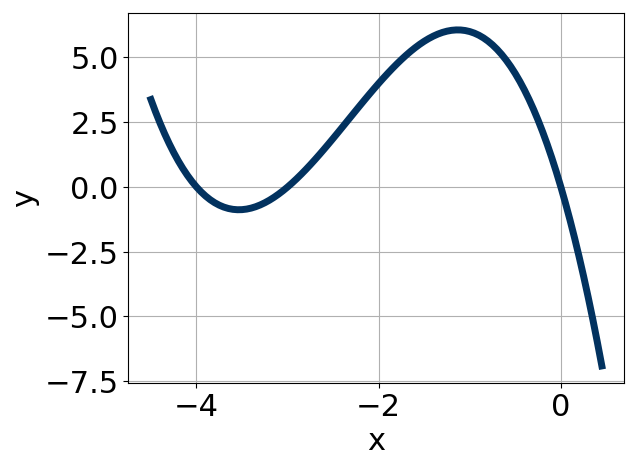
\includegraphics[width=0.3\textwidth]{../Figures/polyGraphToFunctionA.png} \end{center} 

The solution is $ -12x^{7} (x + 4)^{11} (x + 3)^{5} $ 

\begin{enumerate}[label=\Alph*.] 
\item $ 3x^{11} (x + 4)^{9} (x + 3)^{7} $ 

 This corresponds to the leading coefficient being the opposite value than it should be. 
\item $ -16x^{5} (x + 4)^{6} (x + 3)^{9} $ 

 The factor $-4$ should have been an odd power. 
\item $ 13x^{7} (x + 4)^{8} (x + 3)^{11} $ 

 The factor $(x + 4)$ should have an odd power and the leading coefficient should be the opposite sign. 
\item $ -12x^{7} (x + 4)^{11} (x + 3)^{5} $ 

 * This is the correct option. 
\item $ -8x^{7} (x + 4)^{4} (x + 3)^{10} $ 

 The factors $-4$ and $-3$ have have been odd power. 
\end{enumerate} 
 
General Comments: Draw the x-axis to determine which zeros are touching (and so have even multiplicity) or cross (and have odd multiplicity).

-----------------------------------------------

27. Construct the lowest-degree polynomial given the zeros below. Then, choose the intervals that contain the coefficients of the polynomial in the form $x^3+bx^2+cx+d$.
$$ 2 + 5i \text{ and } -1 $$ 
The solution is $ x^{3} -3 x^{2} +25 x + 29 $ 

\begin{enumerate}[label=\Alph*.] 
\item $ b \in [0.34, 1.62], c \in [-2.4, 2], \text{ and } d \in [-2.7, -1.7] $ 

 $x^{3} + x^{2} -x -2$, which corresponds to multiplying out $(x -2)(x + 1)$. 
\item $ b \in [0.34, 1.62], c \in [-4.5, -2.8], \text{ and } d \in [-6.2, -2.6] $ 

 $x^{3} + x^{2} -4 x -5$, which corresponds to multiplying out $(x -5)(x + 1)$. 
\item $ b \in [2.13, 4.2], c \in [22.8, 25.3], \text{ and } d \in [-31.7, -26.8] $ 

 $x^{3} +3 x^{2} +25 x -29$, which corresponds to multiplying out $(x-(2 + 5i))(x-(2 - 5i))(x -1)$. 
\item $ b \in [-4, -2.79], c \in [22.8, 25.3], \text{ and } d \in [25.8, 29.8] $ 

 * $x^{3} -3 x^{2} +25 x + 29$, which is the correct option. 
\item $ \text{None of the above.} $ 

 This corresponds to making an unanticipated error or not understanding how to use nonreal complex numbers to create the lowest-degree polynomial. If you chose this and are not sure what you did wrong, please contact the coordinator for help. 
\end{enumerate} 
 
General Comments: Remember that the conjugate of $a+bi$ is $a-bi$. Since these zeros always come in pairs, we need to multiply out $(x-(2 + 5i))(x-(2 - 5i))(x-(-1))$.

-----------------------------------------------

28. Construct the lowest-degree polynomial given the zeros below. Then, choose the intervals that contain the coefficients of the polynomial in the form $ax^3+bx^2+cx+d$.
$$ \frac{-1}{3}, \frac{6}{5}, \text{ and } \frac{-4}{5} $$ 
The solution is $ 75x^{3} -5 x^{2} -82 x -24 $ 

\begin{enumerate}[label=\Alph*.] 
\item $ a \in [73, 89], b \in [-9, -3], c \in [-92, -72], \text{ and } d \in [-25, -23] $ 

 * $75x^{3} -5 x^{2} -82 x -24$, which is the correct option. 
\item $ a \in [73, 89], b \in [-1, 6], c \in [-92, -72], \text{ and } d \in [23, 30] $ 

 $75x^{3} +5 x^{2} -82 x + 24$, which corresponds to multiplying out $(3x -1)(5x + 6)(5x -4)$. 
\item $ a \in [73, 89], b \in [-9, -3], c \in [-92, -72], \text{ and } d \in [23, 30] $ 

 $75x^{3} -5 x^{2} -82 x + 24$, which corresponds to multiplying everything correctly except the constant term. 
\item $ a \in [73, 89], b \in [-58, -52], c \in [-64, -57], \text{ and } d \in [23, 30] $ 

 $75x^{3} -55 x^{2} -62 x + 24$, which corresponds to multiplying out $(3x + 3)(5x -5)(5x -5)$. 
\item $ a \in [73, 89], b \in [124, 136], c \in [16, 26], \text{ and } d \in [-25, -23] $ 

 $75x^{3} +125 x^{2} +22 x -24$, which corresponds to multiplying out $(3x + 3)(5x + 5)(5x -5)$. 
\end{enumerate} 
 
General Comments: To construct the lowest-degree polynomial, you want to multiply out $(3x + 1)(5x -6)(5x + 4)$

-----------------------------------------------

29. Describe the zero behavior of the zero $x = -5$ of the polynomial below.
$$ f(x) = 4(x + 8)^{4}(x - 8)^{2}(x + 5)^{7}(x - 5)^{4} $$ 

 
 The solution is  
 \begin{center} 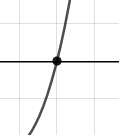
\includegraphics[width=0.3\textwidth]{../Figures/zeroBehaviorPositiveOddA.png} \end{center}\begin{tabular}{|c|c|} 
\hline 
 & \tabularnewline 
 \textbf{A.} 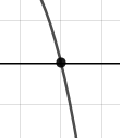
\includegraphics[width=0.3\textwidth]{../Figures/zeroBehaviorNegativeOddA.png} & \textbf{B.} 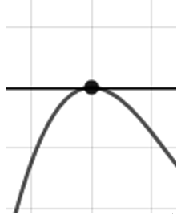
\includegraphics[width=0.3\textwidth]{../Figures/zeroBehaviorNegativeEvenA.png} \tabularnewline 
\hline 
 & \tabularnewline 
 \textbf{C.} 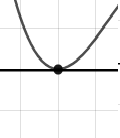
\includegraphics[width=0.3\textwidth]{../Figures/zeroBehaviorPositiveEvenA.png} & \textbf{D.} 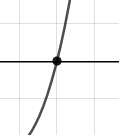
\includegraphics[width=0.3\textwidth]{../Figures/zeroBehaviorPositiveOddA.png} \tabularnewline 
\hline 
 E. None of the figures above. & \tabularnewline 
\hline 
 \end{tabular} 
 
\textbf{General Comments:} You will need to sketch the entire graph, then zoom in on the zero the question asks about.

-----------------------------------------------

30. Describe the end behavior of the polynomial below.
$$ f(x) = -3(x - 5)^{3}(x + 5)^{4}(x - 6)^{5}(x + 6)^{7} $$ 

 
 The solution is  
 \begin{center} 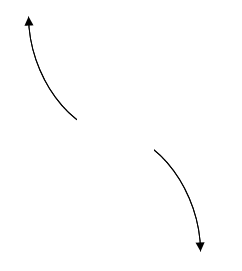
\includegraphics[width=0.3\textwidth]{../Figures/endBehaviorNegativeOddA.png} \end{center}\begin{tabular}{|c|c|} 
\hline 
 & \tabularnewline 
 \textbf{A.} 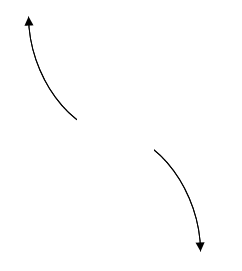
\includegraphics[width=0.3\textwidth]{../Figures/endBehaviorNegativeOddA.png} & \textbf{B.} 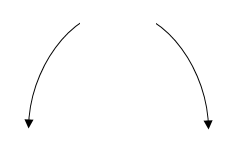
\includegraphics[width=0.3\textwidth]{../Figures/endBehaviorNegativeEvenA.png} \tabularnewline 
\hline 
 & \tabularnewline 
 \textbf{C.} 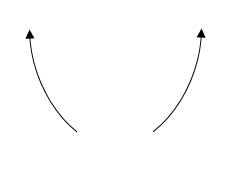
\includegraphics[width=0.3\textwidth]{../Figures/endBehaviorPositiveEvenA.png} & \textbf{D.} 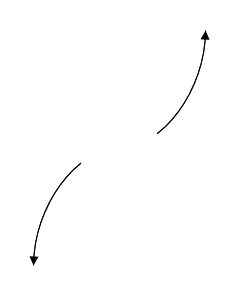
\includegraphics[width=0.3\textwidth]{../Figures/endBehaviorPositiveOddA.png} \tabularnewline 
\hline 
 E. None of the figures above. & \tabularnewline 
\hline 
 \end{tabular} 
 
\textbf{General Comments:} Remember that end behavior is determined by the leading coefficient AND whether the \textbf{sum} of the multiplicities is positive or negative.

-----------------------------------------------


\end{document}

